%!TEX root = <main.tex>
\section{Experimental Evaluation}

\subsection{End-to-End Evaluation}

\subsection{Drill-Down Analysis}

\begin{figure}[t]
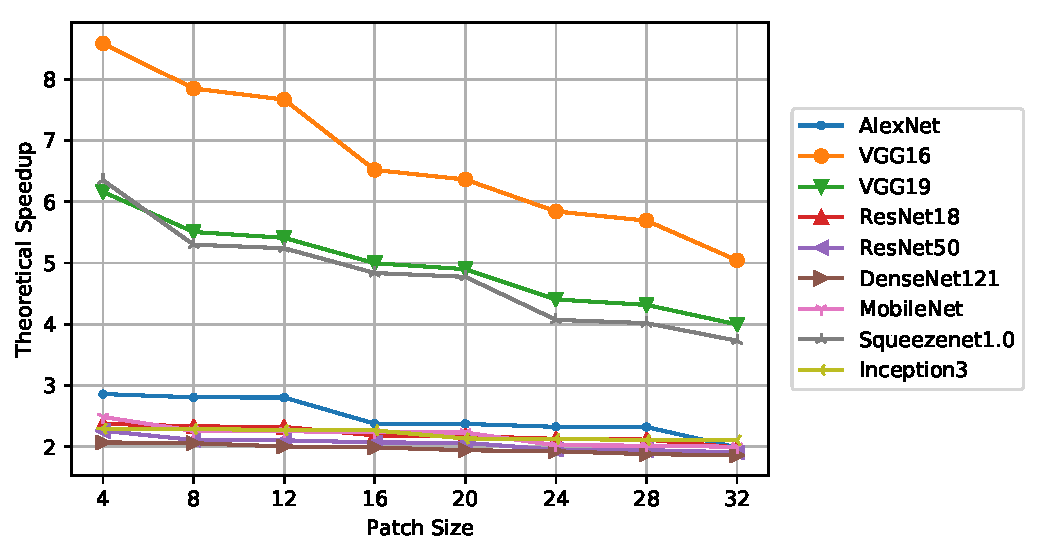
\includegraphics[width=\columnwidth]{images/redundancy_ratio}
\caption{Maximum attainable redundancy ratios of popular CNN architectures when a square occlusion patch of different sizes is placed on the center of the image.}
\label{fig:redundancy_ratio}
\end{figure}

Figure \ref{fig:redundancy_ratio} shows how the maximum attainable redundancy ratio changes for popular CNN architectures when a square occlusion patch of different sizes is placed on the center\footnote{If the occlusion patch is placed towards to a corner of the input image the redundancy ratio will be slightly higher. But placing the occlusion on the center gives us a worst case estimate.} of the input image. VGG 16 layer version results in the maximum redundancy ratio and Inception V3 model has the lowest redundancy ratio. Most CNN architectures results in a redundancy ratio between 2-3 except VGG 16, VGG 19, and Squeezenet 1.0 CNNs which results in higher redundancy ratios. The attainable redundancy ratio of a CNN is determined by the aspects of it's internal architecture such as number of layers, the size of the filter kernels, and the filter stride values.
